\chapter{Quantum Simulation of PDEs: Schr\"odingerization}\label{ch:sec05}

\section{Schr\"odingerization of the heat equation}\label{sec:sec05-schrod}

Consider the heat equation
\begin{equation}
  \partial_t u - \Delta u = 0, \qquad u(0, x) = u_0(x),
  \qquad x = (x_1, \dots, x_d) \in \R^d,\ t \ge 0.
\end{equation}
Introduce an auxiliary variable $p \ge 0$ and define
\begin{equation}
  w(t, x, p) = \ee^{-p} u(t, x), \qquad p \ge 0.
  \label{eq:sec05-warp}
\end{equation}
A simple calculation shows that
\begin{equation}
  \partial_t w = -\partial_p \Delta_x w, \qquad p \ge 0.
\end{equation}
From $w$, $u$ can be recovered by
\begin{equation}
  u(t, x) = \int_0^\infty w(t, x, p)\,\dd p = \int_{-\infty}^\infty \chi(p)\, w(t, x, p)\,\dd p,
  \qquad \chi(p) = \begin{cases} 1 & p > 0, \\ 0 & p \le 0, \end{cases}
\end{equation}
or, since $u(t, x) = \ee^{p} w(t, x, p)$ for all $p \ge 0$, one simply chooses any
$p_* > 0$ and lets $u(t, x) = \ee^{p_*} w(t, x, p_*)$.

Apply the Fourier transform on $x$ (assume $x$ is defined in a periodic domain)
and let $\hat{w}(t, \xi, p)$ be the Fourier transform of $w$, with
$\xi = [\xi_1, \dots, \xi_d]^{\mathsf{T}}$ the Fourier modes:
\begin{equation}
  \partial_t \hat{w} - \abs{\xi}^2 \partial_p \hat{w} = 0,
  \qquad \abs{\xi}^2 = \xi_1^2 + \cdots + \xi_d^2.
\end{equation}
This is an advection equation with the solution going from right to left. Since
the initial data of $w$ is given by $w(0, x, p) = \ee^{-p} u_0(x)$ for $p \ge 0$,
no boundary condition is needed at $p = 0$. Moreover, if we extend $w$ to $p < 0$,
it does not impact the region $p \ge 0$ for $w$. For this reason, we symmetrically
extend the initial data of $w$ to $p < 0$:
\begin{equation}
  \begin{cases}
    \partial_t w + \Delta_x \partial_p w = 0, & p \in (-\infty, \infty), \\
    w(0, x, p) = \ee^{-\abs{p}} u_0(x). &
  \end{cases}
  \label{eq:sec05-extended}
\end{equation}
(There exist other ways of extension.) For $p \ge 0$, the solution coincides with
the solution of \eqref{eq:sec05-warp}. Due to the exponential decay of
$\ee^{-\abs{p}}$, one can impose the periodic boundary condition
$w(t, x, p = -L) = w(t, x, p = L)\ (= 0)$ in the $p$ direction for $L > 0$
sufficiently large. The Fourier transform on $p$ gives
\begin{equation}
  \partial_t \tilde{w} - \ii\eta\Delta\tilde{w} = 0
  \qquad\text{or}\qquad \ii\partial_t \tilde{w} = -\eta\Delta\tilde{w},
  \label{eq:sec05-schrod-eq}
\end{equation}
where $\tilde{w}(t, x, \eta)$, $\eta \in \R$, is the Fourier transform of $w$ in
$p$. Equation \eqref{eq:sec05-schrod-eq} is clearly a Schr\"odinger equation for
every $\eta$.

Here $\tilde{w}$ evolves according to
$\tilde{w}(t, x, \eta) = \exp(-\ii t\eta\Delta)\tilde{w}(0, x, \eta)$. We embed
$\tilde{w}(0, x, \eta)$ into the amplitudes --- a quantum state
$\ket{\tilde{w}(0)}$. Then we can recover
\begin{equation}
  \ket{\tilde{w}(t)} = \exp(-\ii\, \hat{p}^2 \otimes \hat{\eta}\, t)\ket{\tilde{w}(0)}
\end{equation}
with the unitary quantum operator $\exp(-\ii\, \hat{p}^2 \otimes \hat{\eta}\, t)$,
where $\hat{p} = -\ii\tfrac{\partial}{\partial x}$ is the momentum operator and
$\hat{\eta}$ is the quadrature operator with eigenvalue $\eta$. The overall
procedure is shown in \cref{fig:sec05-embedding}.

\begin{figure}[ht]
  \centering
  \begin{quantikz}
    \lstick{$\ket{w(0)}$} & \gate{\hat{F}} & \gate{\ee^{-\ii H \otimes \hat{\eta}\, t}} & \gate{\hat{F}^\dagger} & \gate{\hat{P}} & \rstick{$\ket{u(t)}$}
  \end{quantikz}
  \caption{Schr\"odingerization: from $\ket{u(0)}$ one forms the product state
    $\ee^{-\abs{p}}\ket{+}$ to obtain $\ket{w(0)}$, applies the QFT
    $\hat{F}$ with respect to $p$, evolves under the unitary
    $\ee^{-\ii H \otimes \hat{\eta}\, t}$, applies the inverse QFT
    $\hat{F}^\dagger$, and finally projects ($\hat{P}$) onto the auxiliary modes
    with $p > 0$ to recover $\ket{u(t)}$.}
  \label{fig:sec05-embedding}
\end{figure}

\paragraph{Justification of \eqref{eq:sec05-extended}.}
Applying the Fourier transform on $x$ to \eqref{eq:sec05-extended} gives
\begin{equation}
  \partial_t \hat{w}(t, \xi, p) - \abs{\xi}^2 \partial_p \hat{w}(t, \xi, p) = 0,
  \quad p \in (-\infty, \infty), \qquad \hat{w}(0, \xi, p) = \ee^{-\abs{p}}\hat{u}_0(\xi),
\end{equation}
with analytical solution
\begin{equation}
  \hat{w}(t, \xi, p) = \hat{w}(t, p + \abs{\xi}^2 t) = \ee^{-\abs{p + \abs{\xi}^2 t}}\hat{u}_0(\xi).
\end{equation}
If $p \ge 0$, then
$\hat{w}(t, \xi, p) = \ee^{-p}\bigl[\ee^{-\abs{\xi}^2 t}\hat{u}_0(\xi)\bigr]$, and the
inverse transform gives
\begin{equation}
  w(t, p) = \ee^{-p}\, \mathcal{F}^{-1}\bigl[\ee^{-\abs{\xi}^2 t}\hat{u}_0(\xi)\bigr] = \ee^{-p} u(t, x).
\end{equation}

\section{Numerical implementation}\label{sec:sec05-numerics}

\begin{example}
Consider $u_t - u_{xx} = 0$ on $x \in (-1, 1)$, $u(0, x) = u_0(x)$, with periodic
boundary conditions $u(t, -1) = u(t, 1)$ and $u_x(t, -1) = u_x(t, 1)$, whose exact
solution is $u(t, x) = \ee^{-\pi^2 t}\sin(\pi x)$.
\end{example}

For the numerical implementation, introduce $\alpha = \alpha(p)$ for $p < 0$:
\begin{equation}
  \begin{cases}
    \partial_t w + \partial_{xxp} w = 0, & p \in (-\infty, \infty), \\
    w(0, x, p) := w_0(x, p) = \ee^{-\alpha\abs{p}} u_0(x). &
  \end{cases}
\end{equation}
To match the exact solution, $\alpha(p) = 1$ for $p > 0$; also truncate at
$p = R$ with $\ee^{-R}$ sufficiently small, and choose a large $\alpha$ for
$p < 0$. Since $\tilde{w}$ moves to the left, choose the artificial boundary at
$p = L \le 0$ for $\abs{L}$ large enough, such that $w$ --- initially almost
compactly supported on $[L_0, R]$ --- will not reach $p = L$ during the
computation.

A Fourier spectral method is used for the discretization. Let $M, N$ be two even
numbers, with step sizes $\Delta x = \tfrac{2}{M}$ (spatial variable) and
$\Delta p = \tfrac{R - L}{N}$ (auxiliary variable), and grids
$-1 = x_0 < x_1 < \cdots < x_M = 1$, $L = p_0 < p_1 < \cdots < p_N = R$. Let
$w(t, p) = [w(t, x_0, p), \dots, w(t, x_M, p)]^{\mathsf{T}}$. The discrete Fourier
transform (DFT) on $x$ gives
\begin{equation}
  \begin{cases}
    \partial_t w(t, p) - \hat{P}_\mu^2 \partial_p w(t, p) = 0, & p \in (L, R), \\
    w(0, p) = \ee^{-\alpha\abs{p}} u_0, &
  \end{cases}
\end{equation}
where $\hat{P}_\mu$ is the matrix representation of the moment operator
$-\ii\partial_x$ and $u_0 = [u(0, x_1), \dots, u(0, x_M)]^{\mathsf{T}}$.

The matrix $\hat{P}_\mu$ can be diagonalized as
$D_\mu = \Phi^{-1}\hat{P}_\mu\Phi$, where
$D_\mu = \diag(\mu_{-M/2}, \dots, \mu_{M/2-1})$ is a diagonal matrix with
$\mu_l = \pi l$, $l = -\tfrac{M}{2}, \dots, \tfrac{M}{2} - 1$. Let
$\hat{w}(t, p) = \Phi^{-1} w(t, p)$; then
\begin{equation}
  \partial_t \hat{w}(t, p) - D_\mu^2 \partial_p \hat{w}(t, p) = 0, \quad p \in (L, R),
  \qquad \hat{w}(0, p) = \ee^{-\alpha\abs{p}}\hat{u}_0,
\end{equation}
where $\hat{u}_0 = \Phi^{-1} u_0$.

\begin{figure}[ht]
  \centering
  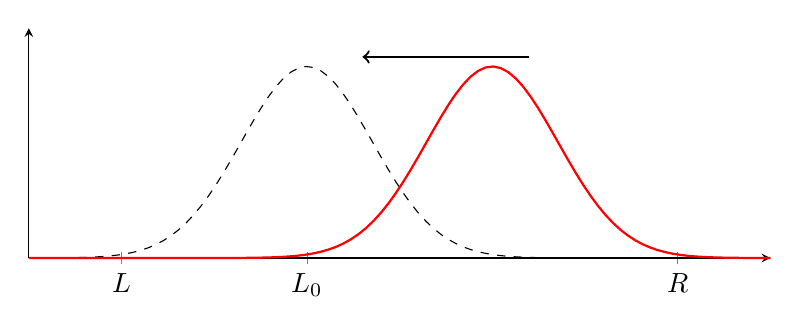
\begin{tikzpicture}
    \begin{axis}[
      width=11cm, height=4.5cm, axis lines=left, ymin=0, ymax=1.2,
      xtick={-3,-1,3}, xticklabels={$L$,$L_0$,$R$}, ytick=\empty,
      xmin=-4, xmax=4, clip=false]
      \addplot[dashed, domain=-4:4, samples=100] {exp(-(x+1)^2)};
      \addplot[red, thick, domain=-4:4, samples=100] {exp(-(x-1)^2)};
      \draw[->, thick] (axis cs:1.4,1.05) -- (axis cs:-0.4,1.05);
    \end{axis}
  \end{tikzpicture}
  \caption{The auxiliary profile (solid, red) is initially almost compactly
    supported on $[L_0, R]$ and moves to the left during evolution (dashed);
    the artificial boundary at $p = L$ is chosen far enough that the profile
    never reaches it.}
  \label{fig:sec05-spectral}
\end{figure}

\subsection{Full discretization}\label{sec:sec05-full}

Consider $W(t) := (w(t, x_i, p_j))_{M \times N}$, which can be straightened as a
column vector
\begin{equation}
  w(t) = [w_0; w_1; \dots; w_{M-1}] = \sum_{ij} w(t, x_i, p_j)\ket{i, j},
  \qquad w_i = [w(t, x_i, p_0), \dots, w(t, x_i, p_{N-1})]^{\mathsf{T}}.
\end{equation}
Performing the DFT on both $x$ and $p$ yields
\begin{equation}
  \partial_t w(t) - \ii\bigl(\hat{P}_\mu^2 \otimes \hat{P}_\mu\bigr) w(t) = 0
\end{equation}
(using $\hat{P}_\mu$ for both the $x$ and $p$ variables). In the frequency space,
let $c(t) = (F_x^{-1} \otimes F_p^{-1}) w(t)$; then
\begin{equation}
  \partial_t c(t) - \ii\bigl(D_\mu^2 \otimes D_\mu\bigr) c(t) = 0.
\end{equation}

\section{Heat equation with a source term}\label{sec:sec05-source}

Consider $\partial_t u - \Delta u = V(x) u$, $u(0, x) = u_0(x)$. Using the
previous notation, $\partial_p w = \ii(-\ii\partial_p w) \to \ii\hat{P}_\mu w(t, x)$
where $w(t, x) = [w(t, x, p_0), w(t, x, p_1), \dots, w(t, x, p_{N-1})]^{\mathsf{T}}$.
We have the semi-discrete system of PDEs
\begin{equation}
  \partial_t w(t, x) + \ii[\Delta_x + V(x)]\hat{P}_\mu w(t, x) = 0,
  \qquad w(0, x) = w_0(x) := [w_0(x, p_j)]_{N \times 1}.
\end{equation}
In the moment basis, one has
\begin{equation}
  \partial_t c(t, x) + \ii[\Delta_x + V(x)] D_\mu\, c(t, x) = 0,
  \qquad c(0, x) = c_0(x) := \Phi^{-1} w_0(x),
\end{equation}
where $c = F_p^{-1} w$. The above PDEs can be viewed as a quantum system.

\subsection{Quantum simulation of the heat equation}\label{sec:sec05-heat-sim}

Let $w(t, x, p) = \sum_l c_l(t)\phi_l(x, p)$, $l = (l_1, \dots, l_d, l_p)$. The
collocation points are denoted by $(x_j, p_p)$ with $j = (j_1, \dots, j_d)$.
Define $c = c_x \otimes c_p$, where $c_x = c^{(1)} \otimes \cdots \otimes c^{(d)}$.
We also introduce $w = w_x \otimes w_p$, where
$w_x = w^{(1)} \otimes \cdots \otimes w^{(d)}$ and $w^{(l)} = \Phi\, c^{(l)}$. Then
\begin{align}
  \Delta_x w_p &= \sum_{l=1}^d \partial_{x_l}^2 \partial_p w
    = -\ii\sum_{l=1}^d (-\ii\partial_{x_l})^2(-\ii\partial_p) w
    = -\ii\sum_{l=1}^d \hat{P}_l^2 \hat{P}_p w \notag\\
  &= -\ii\sum_{l=1}^d (\hat{P}_l^2 \otimes I)(I^{\otimes d} \otimes \hat{P}_p)(w_x \otimes w_p)
    = -\ii\sum_{l=1}^d (\hat{P}_l^2 \otimes \hat{P}_p) w,
\end{align}
where $\hat{P}_l = I^{\otimes(l-1)} \otimes \hat{P} \otimes I^{\otimes(d-l)}$, and
\begin{equation}
  V(x) w_p = \ii V(x)(-\ii\partial_p) w \to \ii V(x^{(d)})\hat{P}_p w
  = \ii(V \otimes I)(I^{\otimes d} \otimes \hat{P}_p)(w_x \otimes w_p) = \ii(V \otimes \hat{P}_p) w,
\end{equation}
where $V$ is a diagonal matrix with $V_{n_j, n_j} = V(x_j)$ and
$n_j = j_1 2^{d} + \cdots + j_d 2^0$. The resulting ODEs are
\begin{equation}
  \frac{\dd}{\dd t} w(t) - \ii\bigl[(\hat{P}_1^2 + \cdots + \hat{P}_d^2 - V) \otimes \hat{P}_p\bigr] w(t) = 0,
\end{equation}
which is the expected Hamiltonian system and can be solved, for example, by
Trotter splitting.

In the moment basis, $\tfrac{\dd}{\dd t}\hat{w}(t) = \ii H\hat{w}(t)$ with
$H = (\hat{P}_1^2 + \cdots + \hat{P}_d^2 - V) \otimes D_\mu$. From $t_n$ to
$t_{n+1}$, split the evolution into two steps:
\begin{enumerate}
  \item Solve $\tfrac{\dd}{\dd t}\hat{w}(t) = \ii[(\hat{P}_1^2 + \cdots + \hat{P}_d^2) \otimes D_\mu]\hat{w}(t)$,
    $t_n < t < t_{n+1}$, with $\hat{w}(t_n) = \hat{w}^n$. Letting
    $\tilde{c}(t) = (F_x^{-1} \otimes I)\hat{w}(t)$, we instead solve
    $\tfrac{\dd}{\dd t}\tilde{c}(t) = \ii H_D \tilde{c}(t)$ with
    $\tilde{c}(t_n) = \tilde{c}^n = (F_x^{-1} \otimes I)\hat{w}^n$, where
    $H_D = [(D_1^\mu)^2 + \cdots + (D_d^\mu)^2] \otimes D_\mu$ is a diagonal
    matrix; denote the numerical solution by $\tilde{c}^*$.
  \item Let $\hat{w}^* = (F_x \otimes I)\tilde{c}^*$, and solve
    $\tfrac{\dd}{\dd t}\hat{w}(t) = -\ii(V \otimes D_\mu)\hat{w}(t) =: -\ii H_V\hat{w}(t)$
    for one time step, with initial data $\hat{w}^*$, giving $\hat{w}^{n+1}$.
\end{enumerate}

\paragraph{Complexity analysis.}
Let $m$ be the number of qubits per dimension, $m_H$ the total number of qubits
with $m_H = m_d + m_p$ and $m_d = dm$, $m_p$ the number of qubits on the $p$
register, and $m_d$ the number of qubits on the $x$ registers. Let
$\Delta x, \Delta p, \Delta t$ be the step sizes for $x, p, t$, so that
$m \sim \log(1/\Delta x)$ and $m_p \sim \log(1/\Delta p)$. For a given error bound
$\varepsilon$, $\Delta t \sim \varepsilon$, $\Delta p \sim \varepsilon$,
$\Delta x \sim (\varepsilon/d)^l$; due to the regularity of the initial condition
on $p$, there is first-order accuracy on $p$.

\begin{theorem}
The solution of the heat equation can be simulated with gate complexity
\begin{equation}
  N_{\mathrm{gates}} = \frac{T}{\Delta t}\, \bigo\bigl(dm\log m + m_p \log m_p\bigr),
\end{equation}
where $T$ is the evolution time.
\end{theorem}

\begin{proof}
Given the initial state $\hat{w}^0$, apply the inverse QFT to the $x$-register to
get $\tilde{c}^0$. At each time step,
\begin{equation}
  \tilde{c}^n \xrightarrow{\ee^{\ii H_D \Delta t}} \tilde{c}^*
  \xrightarrow{F_x^{-1} \otimes I} \hat{w}^*
  \xrightarrow{\ee^{-\ii H_V \Delta t}} \hat{w}^{n+1}
  \xrightarrow{F_x^{-1} \otimes I} \tilde{c}^{n+1},
  \qquad F_x = \Phi^{\otimes d}.
\end{equation}
The QFT in one dimension can be implemented using $\bigo(m\log m)$ gates. The
diagonal unitary operators $\ee^{-\ii H_V \Delta t}$ and $\ee^{\ii H_D \Delta t}$
can be implemented using $\bigo(m_H)$ gates. Therefore the gate complexity up to
the $n$-th step is
\begin{equation}
  N_{\mathrm{gates}} = n\,\bigo(dm\log m + m_p\log m_p + m_H)
  = \frac{T}{\Delta t}\,\bigo(dm\log m + m_p\log m_p),
\end{equation}
where the QFT on the $p$-register is performed twice.
\end{proof}

\section{General linear ODEs}\label{sec:sec05-linear-ode}

Suppose one needs to solve
\begin{equation}
  \frac{\dd u(t)}{\dd t} = A u(t) + b(t), \qquad u(0) = u_0,
\end{equation}
with $A$ independent of time and $A\dg \neq A$. It suffices to assume
$b(t) \equiv 0$; otherwise one can consider the augmented system
\begin{equation}
  \frac{\dd \tilde{u}(t)}{\dd t} = \tilde{A}\tilde{u}(t), \quad \tilde{u}(0) = \tilde{u}_0,
  \qquad \tilde{u} = \begin{psmallmatrix} u \\ v \end{psmallmatrix},\ \tilde{u}_0 = \begin{psmallmatrix} u_0 \\ 1 \end{psmallmatrix},
  \qquad \tilde{A} = \begin{psmallmatrix} A & b(t) \\ 0^{\mathsf{T}} & 0 \end{psmallmatrix}.
\end{equation}

\begin{remark}
A unitary ODE with time-dependent $A(t)$ (non-autonomous) can also be turned into
an autonomous system in one higher dimension (Cao, Jin, Lin, arXiv:2312.02817).
\end{remark}

Let $A = H_1 + \ii H_2$, with
$H_1 = \tfrac{A + A\dg}{2} = H_1\dg$ and $H_2 = \tfrac{A - A\dg}{2\ii} = H_2\dg$.
Then $H_1 H_2 = H_2 H_1$ holds iff $A\dg A = A A\dg$. Assume $H_1$ is negative
semidefinite for stability. It is simple to see that
$2s(H_1) \sim s(A) \sim 2s(H_2)$ (sparsity), and
$\norm{H_1}_{\max}, \norm{H_2}_{\max} \le \norm{A}_{\max}$, which denotes the
largest entry of $A$ in absolute value.

Using the warped phase transformation $v(t, p) = \ee^{p} u(t)$ for $p > 0$ and
symmetrically extending the initial data to $p < 0$,
\begin{equation}
  \begin{cases}
    \dfrac{\dd v(t, p)}{\dd t} = A v(t, p) = -H_1 \partial_p v + \ii H_2 v, \\[0.5em]
    v(0, p) = \ee^{-\abs{p}} u_0.
  \end{cases}
\end{equation}
Then $u(t)$ can be restored by $u(t) = \int_0^\infty v(t, p)\,\dd p$. Applying the
DFT on $p$ gives
\begin{equation}
  \frac{\dd}{\dd t} w(t) = -\ii(H_1 \otimes \hat{P}_\mu) w + \ii(H_2 \otimes I) w,
\end{equation}
where $w = [w_1; w_2; \dots; w_n]$ and $w_i = \sum_k v_i(t, p_k)\ket{k}$. By the
change of variables $\tilde{w} = (I_n \otimes F_p^{-1}) w$, one has
\begin{equation}
  \frac{\dd}{\dd t} \tilde{w}(t) = -\ii(H_1 \otimes D_\mu)\tilde{w} + \ii(H_2 \otimes I)\tilde{w}.
\end{equation}

\begin{definition}[Sparse access]
Let $A$ be a Hermitian matrix with $(j,k)$-th entry $A_{jk}$. Sparse access to $A$
is a $4$-tuple $(s, \norm{A}_{\max}, O_A, O_F)$, where $O_A$ is a unitary oracle
that accesses $A_{jk}$ such that
$O_A\ket{j}\ket{k}\ket{z} = \ket{j}\ket{k}\ket{z \oplus A_{jk}}$ for all
$j, k \in [N]$ (the third register holds a bit string representing $A_{jk}$), and
$O_F$ is an oracle that allows $O_F\ket{j}\ket{l} = \ket{j}\ket{F(j, l)}$ with
$j \in [N]$, $l \in [s]$, where $F$ outputs the column index of the $l$-th nonzero
entry in row $j$.
\end{definition}

\begin{lemma}[Berry, Childs, Kothari, 2015]
An $s$-sparse Hamiltonian $H$ acting on $m_H$ qubits can be simulated within
error $\varepsilon$ with
\begin{equation}
  \bigo\!\Bigl(\tau\, \frac{\log(\tau/\varepsilon)}{\log\log(\tau/\varepsilon)}\Bigr)
\end{equation}
queries and
\begin{equation}
  \bigo\!\Bigl(\tau\bigl[m_H + \log^{2.5}(\tau/\varepsilon)\bigr]\frac{\log(\tau/\varepsilon)}{\log\log(\tau/\varepsilon)}\Bigr)
  = \bigo(\tau\, m_H\, L_{\mathrm{polylog}})
\end{equation}
additional two-qubit gates, where $\tau = s\norm{H}_{\max} t$, $t$ is the
evolution time, and
$L_{\mathrm{polylog}} = [1 + \log^{2.5}(\tau/\varepsilon)]\frac{\log(\tau/\varepsilon)}{\log\log(\tau/\varepsilon)}$.
This result is nearly optimal.
\end{lemma}

Assume $A$ arises from some discretization in $d$ dimensions, so that
$N_A \sim 2^{m_d}$ with $m_d = dm$ ($m$ qubits in each direction).

\begin{theorem}
The quantum simulation method has gate complexity
\begin{equation}
  N_{\mathrm{gates}, \mathrm{Schr}} = (m_d + m_p)\,\tilde{\bigo}\!\Bigl(\frac{s(A)\norm{A}_{\max} T}{\Delta p}\Bigr) + \bigo(m_p\log m_p),
\end{equation}
where $\tilde{\bigo}$ suppresses all logarithmic factors. In particular, if $H_1$
can be diagonalized in the momentum basis and $H_2$ is a diagonal matrix, then the
method can be implemented with
\begin{equation}
  N_{\mathrm{gates}, \mathrm{Schr}} = \frac{T}{\Delta t}\,\bigo(dm\log m + m_p\log m_p).
\end{equation}
\end{theorem}

\begin{proof}
The Hamiltonian $H = H_1 \otimes D_\mu - H_2 \otimes I$ can be simulated with
complexity
\begin{align}
  &T(m_d + m_p)\tilde{\bigo}\bigl(s(H_1 \otimes D_\mu - H_2 \otimes I)\norm{H_1 \otimes D_\mu - H_2 \otimes I}_{\max}\bigr) \notag\\
  &\quad \le T\tilde{\bigo}\bigl((s(H_1 \otimes D_\mu) + s(H_2 \otimes I))(\norm{H_1 \otimes D_\mu}_{\max} + \norm{H_2}_{\max})\bigr) \notag\\
  &\quad \le T\tilde{\bigo}\bigl((s(H_1) + s(H_2))(\norm{H_1}_{\max}/\Delta p + \norm{H_2}_{\max})\bigr)
  \le \tilde{\bigo}\bigl(s(A)\norm{A}_{\max} T/\Delta p\bigr),
\end{align}
where $\abs{D_\mu}_{\max} \lesssim 1/\Delta p$ is used. For the special case, one
can solve the system by the first-order time-splitting scheme.
\end{proof}

For the heat equation, $\norm{A}_{\max} \sim 1/(\Delta r)^2$, which motivates the
preconditioning issue treated in \cref{ch:sec07}.
